\documentclass[a4paper]{article}
\usepackage{amsmath,amsfonts,amsthm,amssymb}
\usepackage{physics}
\usepackage{geometry}
\usepackage{graphicx}
\title{The Catenary}
\author{Gordon Chan}

\begin{document}
\maketitle
\section{Assumptions and Details}
\begin{itemize}
    \item the catenary has a finite length \(S\)
    \item gravity is uniform and downwards with magnitude \(g\)
    \item the catenary has a uniform linear density \(\rho\) such that
        it has total mass \(m=S\rho\)
    \item the catenary is suspended at its two end points
    that are distance \(0<d<S\) apart horizontally and have the same vertical level
\end{itemize}

\section{Derivation}
To determine the equation of the catenary \(y(x)\), 
let the point \((x,y)\) be a point on the catenary that is distance \(s\) 
along the cable from the lowest point of the catenary. 
Also, let the tangent of the catenary at \((x,y)\) have an angle of \(\theta\)
with respect to the horizontal.
Further let the tension acting on \((x,y)\) be \(T\)
and the tension acting on the lowest point be \(T_x\).

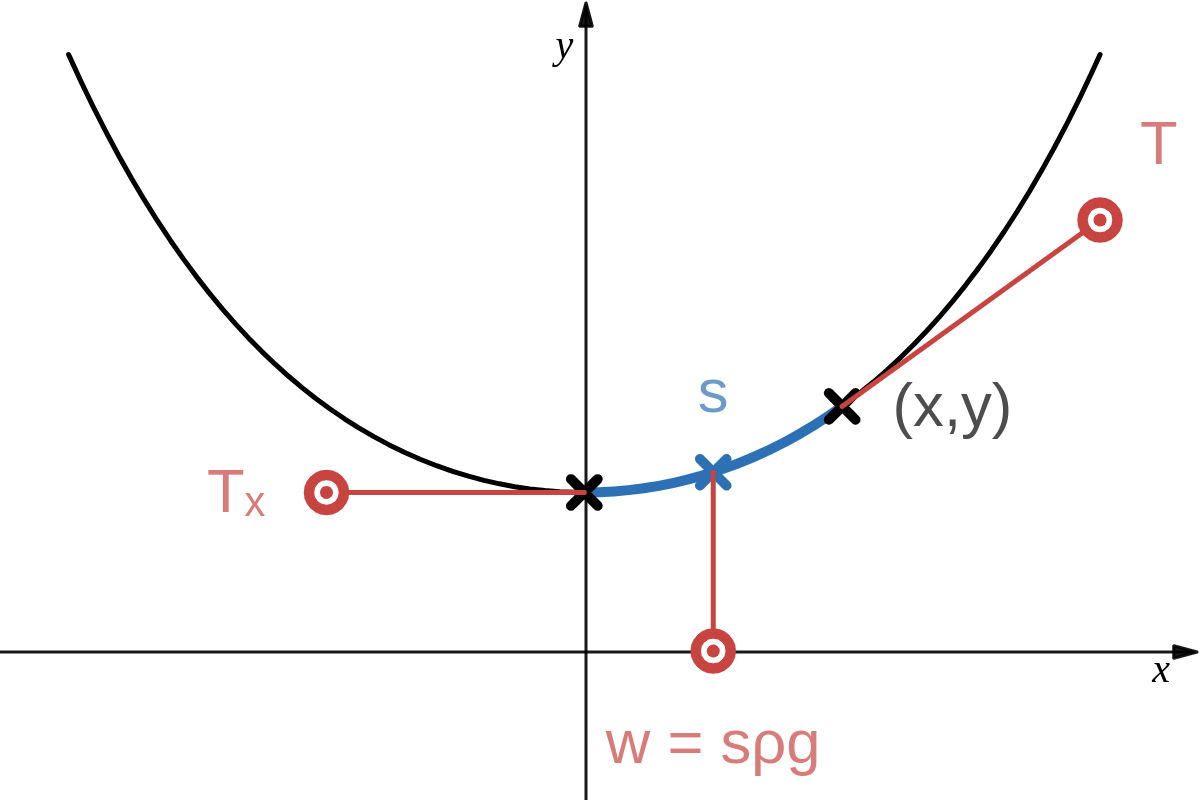
\includegraphics[width=.9\textwidth]{catenary.png}

By equilibrium, it can be deduced that,
\begin{equation}
    \sum F_x=0\implies T\cos\theta-T_x=0\implies T\cos\theta=T_x
\end{equation}

\begin{equation}
    \sum F_y=0\implies T\sin\theta-w=0\implies T\sin\theta=s\rho g
\end{equation}

By dividing the two equations,
\begin{equation}
    \tan\theta=\frac{s\rho g}{T_x}
\end{equation}

Let \(\varphi=\frac{\rho g}{T_x}\). Since at \((x,y)\), \(\dv{y}{x}=\tan\theta\),
\begin{equation}
    \dv{y}{x}=\varphi s
\end{equation}

By the Pythagoras' theorem, 
\begin{equation}
    \dd{s}^2=\dd{x}^2+\dd{y}^2
\end{equation}

By dividing \(\dd{x}^2\) and taking the square root on both sides of the equation,
\begin{equation}
    \dv{s}{x}=\sqrt{1+\pqty{\dv{y}{x}}^2}
\end{equation}

By differentiating the first derivative,
\begin{equation}
    \dv[2]{y}{x}=\varphi\dv{s}{x}
\end{equation}

\begin{equation}
    \dv[2]{y}{x}=\varphi\sqrt{1+\pqty{\dv{y}{x}}^2}
\end{equation}

Let \(m=\dv{y}{x}\),
\begin{equation}
    \dv{m}{x}=\varphi\sqrt{1+m^2}
\end{equation}

\begin{equation}
    \frac1{\sqrt{1+m^2}}\dd{m}=\varphi\dd{x}
\end{equation}

By integrating both sides,
\begin{equation}
    \sinh^{-1}m=\varphi x+C
\end{equation}

By intuition, \(m(0)=0\), thus,
\begin{equation}
    \sinh^{-1}0=\varphi\cdot0+C\implies C=0
\end{equation}

\begin{equation}
    \dv{y}{x}=\sinh\varphi x
\end{equation}

By integration,
\begin{equation}
    y=\frac1\varphi\cosh\varphi x+C
\end{equation}

Let \(a=\frac1\varphi\) and \(b=C\).
\[\therefore\boxed{y(x)=b+a\cosh\frac xa}\]
\end{document}
